\documentclass{article}

\usepackage[most]{tcolorbox}
\usepackage{physics}
\usepackage{graphicx}
\usepackage{amsmath}
\usepackage{amssymb}
\usepackage{float}


\usepackage[utf8]{inputenc}
\usepackage[a4paper, margin=1in]{geometry} % Controla los márgenes
\usepackage{titling}

\title{Clase 3 }
\author{Manuel Garcia.}
\date{\today}

\renewcommand{\maketitlehooka}{%
  \centering
  \vspace*{0.05cm} % Espacio vertical antes del título
}

\renewcommand{\maketitlehookd}{%
  \vspace*{2cm} % Espacio vertical después de la fecha
}

\newcommand{\caja}[3]{%
  \begin{tcolorbox}[colback=#1!5!white,colframe=#1!25!black,title=#2]
    #3
  \end{tcolorbox}%
}

\begin{document}
\maketitle

\section{Curvas en $ \mathbb{R}^2   $ y $ \mathbb{R}^3  $}
\caja{red}{Curvas en $ \mathbb{R}^3   $}{
  \begin{gather}
    r = r(t) \rightarrow x = x(t) \quad y = y(t) \quad \text{r es un vector} 
    \label{eq:curva_r2}
  \end{gather}
  Curvas parametrizadas en función de la longitud de arco
  \begin{gather}
    l = \int_{a }^{b }\sqrt{\dot x^2 + \dot y^2  }dt = \int_{a }^{b }|v_t| dt = \int_{0 }^{l} dl', \quad dl = |v_t|dt 
    \label{eq:param_long_arco}
  \end{gather}
  Tenemos una parametrizacion:
  \begin{gather}
     \frac{d l }{d t} = |v_t | \rightarrow \frac{d t }{d l} = \frac{1}{|v_t|} \leftarrow l = l(t) \rightarrow t = t(l)  
  \end{gather}
}
\begin{gather}
   dl^2 = \bra{v_t }\ket{v_t }dt^2 = (\frac{d x^2  }{d t }+ \frac{d y^2  }{d t^2 }) dt^2 \\
   \bar v_l = \frac{d \bar r  }{d l } = \frac{d \bar r  }{d t }\frac{d t  }{d l } = \frac{\bar v_t }{|v_t|}\\
   dl^2 = v_t^2 dt^2 \\
   \bra{v_l }\ket{v_l} = 1  
\end{gather}
\caja{green}{Aceleracion }{
  \begin{gather}
    \frac{d ^2 r  }{d t^2 } \equiv w_t    
    \label{eq:aceleracion }
  \end{gather}
}
Vamos a suponer que $ \bra{v}\ket{v} = cte  \rightarrow \frac{d  }{d t}\bra{v}\ket{v} = 0  $

\begin{gather}
  \bra{\frac{d u }{d t}  }\ket{v}+\bra{v}\ket{\frac{d u  }{d t}} = 2 \bra{u }\ket{\frac{d u  }{d t}  } = 0 
  \bra{v}\ket{\psi} \\
  \bra{v }\ket{w } = 0 \leftarrow v \text{ortogonal a } w   
\end{gather}
Si $ t = l  $ entonces $v_l$ ortogonal a $w_l$ 

\begin{gather}
   \bra{v_l } \ket{v_l } = 1 \rightarrow \bra{v_l }\ket{w_l } = 0    
\end{gather}
\caja{green}{curvatura }{
  \begin{gather}
    k(l) \equiv |w_l | = |\frac{d ^2 r  }{d l^2 }| = | \frac{d v_l  }{d l }|\\
    R(l)  \equiv \frac{1}{k(l) } \rightarrow \text{Radio de curvatura}   
    \label{eq:curvatura }
  \end{gather}
  n es el vector normal y vamos definir la aceleracion la cual es la curvatura por el vector normal: 
  \begin{gather}
    w_l \equiv k(l)n \qquad \text{n es el vector normal } 
    \label{eq:aceleracion }
  \end{gather}
  Esto es muy util en la mecanica de fluidos ideales que está compuesto por la longitud de arco a lo largo de una linea de flujo y la normal a la misma. 
}
\caja{red}{Radio de curvatura }{
  \begin{gather}
    R(t) \equiv \frac{1}{k(t)}
    \label{eq:radio_curvatura }
  \end{gather}
}

\textbf{Ejemplo: } Linea recta $ x = a+bx, y = c+dl  \rightarrow v_l = be_x + de_y  \rightarrow w_l = 0, |w_l| = 0 \rightarrow k = 0, R = \infty  $

\textbf{Ejemplo: } Circulo $ x = x_0 +R \cos{\frac{l}{R} } , y = y_0 + R \sin{\frac{l}{R} }   $
\begin{gather}
  v_l = (-\cos{\frac{l}{R} }, \sin{\frac{l}{R} }    ) 
  w_i = -\frac{1}{R}\cos{\frac{l}{R} }e_x - \frac{1}{R}\sin{\frac{l}{R} }e_y \rightarrow |w_l| = k(l) = \frac{1}{R},\quad R = \frac{1}{k(l)} = R        
  \label{eq:curvatura_circulo }
\end{gather}

\subsection{Formulas de frenet-serret}
\caja{red}{Frenet-Serret }{
  Para una curva plana parametrizada en fución de la longitud de arco, se cimple las siguientes expresiones. 
  \begin{gather}
    \underset{definicion}{w_l \equiv \frac{d v }{d l} = kn}, \qquad \frac{d n }{d l} = -kv    
    \label{eq:null}
  \end{gather}
  La primera eq nos indica como se comporta la velocidad conforme vamos avanzando en la curva, nos indica la direccion de la velocidad cuando vamos avanzando en la curva.
}
Para ver como se comporta la normal cuando vamos avanzado en la curva:
\begin{gather}
   \bra{v}\ket{n } = 0 \rightarrow \frac{d  }{d l }\bra{v }\ket{n} = \bra{\frac{d v }{d l}  }\ket{n }+\bra{v}\ket{\frac{d n  }{d l}  }\\
   \bra{kn}\ket{n }+\bra{v}\ket{\frac{d n }{d l}  } = k + \bra{v}\ket{\frac{d n }{d l}  } = 0 \rightarrow \bra{v}\ket{\frac{d n }{d l}  } = -k  
\end{gather}
Curvatura:
\begin{gather}
   \frac{d n }{d l} = \alpha n + \beta v \rightarrow \bra{\frac{d n }{d l}  }\ket{v} = \bra{\alpha n +\beta v }\ket{v} = \beta     
\end{gather}
$ \frac{d n }{d l}   $ es proporcional a v entonces $ \beta=-k $
\begin{gather}
   \frac{d n }{d l}=-kv  
\end{gather}

como expansion en series:
\begin{gather}
  v = v_0 + \Delta v = v_0 +\Delta l kn + O(\Delta l^2) \approx v_0 +\Delta \phi n = \cos{\Delta \phi } v_0 + \sin{\Delta\phi } n_0  \\
  n = n_0 + \Delta n = n_0 - \Delta lkv + O(\Delta l^2) \approx n_0-\Delta \phi v = -\sin{\Delta \phi } v_0 +\cos{\Delta\phi } n_0  
  \label{eq:expansion }
\end{gather}
En este punto se utilizo la expansion en serie del seno y el coseno al primer orden. 

Por lo tanto:
\begin{gather}
  \begin{bmatrix}
      v \\
      n 
  \end{bmatrix}  
  =
  \begin{bmatrix}
      \cos{\Delta\phi }   & \sin{\Delta \phi }   \\
      -\sin{\Delta \phi }   & \cos{\Delta \phi }  
  \end{bmatrix} 
  \begin{bmatrix}
      n_0  \\
      v_0  
  \end{bmatrix} |_P \rightarrow k \equiv \frac{d \phi  }{d l}   
  \label{eq:v_n}
\end{gather}

\subsection{Curvatura en función del parámetro t}
\caja{green}{Curvatura en funcion de t }{
  \begin{gather}
    \frac{d v_l  }{d l}=\frac{1}{|v_t| }\left[ -\frac{\bra{v_t }\ket{w_t } }{|v_t|^3 }v + \frac{1}{|v_t|}\frac{d ^2 r  }{d t^2 }     \right]   \\
    k = \frac{1}{|\dot r|^2 }\left|\ddot r - \frac{\bra{\dot r }\ket{\ddot r } }{|\dot r|^2}\right| 
  \end{gather}
  Todo el procedimiento está en las diapositivas.
}
\caja{black}{Ejercicio}{
  Mostrar que en componentes x(t), y(t) la curvatura es:
  \begin{gather}
     k = \frac{|\ddot x \dot y - \ddot y \dot x |}{(\dot x^2 + \dot y^2)^ {3/2}} 
  \end{gather}
}

\section{Curvas en $ \mathbb{R}  $ } % (fold)
El vector binormal es el producto cruz entre el vector normal $ n  $ y el vector de torsion $t$.
\begin{figure}[H]
  \begin{center}
    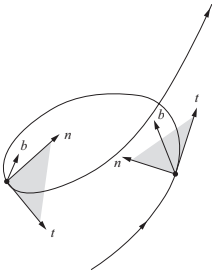
\includegraphics[width=0.2\textwidth]{vector_binormal.png}
  \end{center}
\end{figure}

Ver las propiedades en las diapositivas. 
\begin{figure}[H]
  \begin{center}
    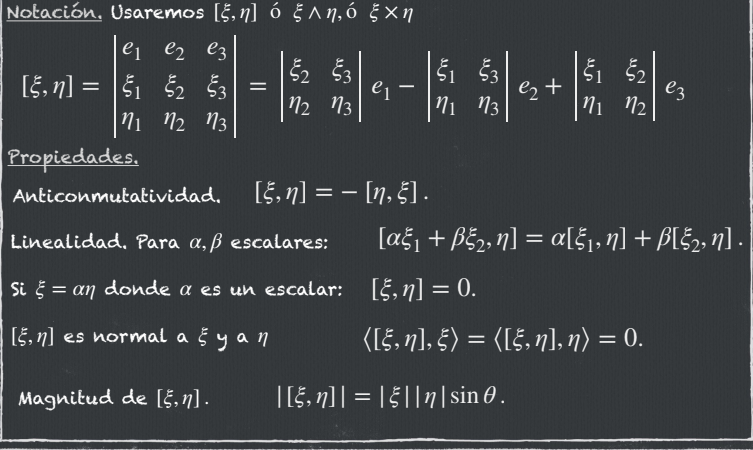
\includegraphics[width=0.85\textwidth]{1.png}
  \end{center}
\end{figure}
\begin{figure}[H]
  \begin{center}
    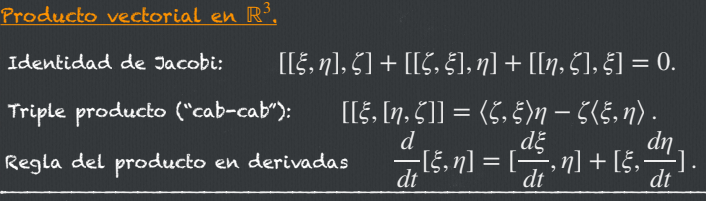
\includegraphics[width=0.85\textwidth]{2.png}
  \end{center}
\end{figure}



% section Curvas en $ \mathbb{R}  $  (end)

\end{document}







